\documentclass[xcolor=svgnames,t,final]{beamer}

\usepackage[T1]{fontenc}
\usepackage[utf8]{inputenc}
\usepackage{lmodern} % Smooth fonts : always use it

\usepackage[french]{babel}

%%%%%%% Page de titre %%%%%%%%%% 

\title{Echantillonnage \\ Corrigés de quelques exemples}\subtitle{Terminale S 734}
\author[]{Frédéric Junier \thanks{\url{http://frederic-junier.org/} }}
\institute[Lycée du Parc]{Lycée du Parc, Lyon}
\date[]{}

%%%%%%Environnements et symboles mathématiques%%%%

%%%Tableaux de variations %%%%%%%%%%

\usepackage{variations}

%%%%%%%%%%%AmsMaths%%%%%%
\usepackage{mathtools}        %Commandes essentielles, extension d'amsmath
\usepackage{amsfonts,amssymb}  %Principaux symboles
\usepackage{mathrsfs} %Polices calligraphiques
\usepackage{stmaryrd} %Pour les intervalles d'entiers avec \llbracket et \rrbracket
\usepackage[autolanguage, np]{numprint}
%%%%%%%%%%%%Là encore il y a de grosses différences entre le monde anglo-saxon et les francophones.Le séparateur des décimales est un point en anglais et une virgule en français. Leséparateur des milliers est une virgule en anglais et une espace insécable en français. Ilest préférable d’utiliser le package numprint (\usepackage{numprint}) qui associé àfrenchb produira la bonne typographie.
%123456789 = 123456789 \numprint{123456789} = 123 456 789  \numprint{3,1415926535897932384626} = 3,141 592 653 589 793 238 462 6  \numprint{12.34} = 12,34  En plus tu peux préciser les unités de cette façon : \numprint[kg]{12.34} = 12,34 kg ou encore \numprint[\degres C]{22} = 22°C Si tu veux utiliser le raccourci \np{} au lieu de \numprint{}, il te faut charger le package de cette façon : \usepackage[np]{numprint}

\usepackage{bbm, dsfont}   %Fonction indicatrice
\usepackage{esint,esvect}  %Flèches supplémentaires.

%%%%url%%%%

\usepackage{url}

%%%%%%%%%%%Packages spécifiques pour les sorties pdf%%%%%%%%

%%%%Insertion de liens hypertextes %%%%

\usepackage{hyperref}
            
            

%%%%%%%%%%%%Graphiques et Dessins%%%%%%%%%%%%%%

\usepackage{graphicx}		
%\rotatebox[origin=x0x1]{angle}{texte} avec xox1 parmi t (top) l (left) r (right) B (ligne de base) et b (bottomm)
%\resizebox{largeur}{hauteur}{texte} pour faire rentrer u nelement encombrant dans une boite	


%%%%%%%%%%Parametrages Beamer %%%%%%%%%%%%%%%%%

\usetheme{Singapore} % Beamer theme
\usecolortheme[named=Purple]{structure} % Color: latextemplates.com/svgnames-colors
\setbeamercolor{navigation symbols}{fg=black}
\setbeamertemplate{navigation symbols}{\insertframenumber}

%À mettre dans le préambule pour faire apparaitre le plan à chaque section 

\AtBeginSection
{
\begin{frame}
\frametitle{Plan}
\tableofcontents[current, currentsubsection]
\end{frame}
}
 

%%%%%%%%%%%%%%%%%%%%%%%%%%%%
%Le moteur eTeX est aujourd'hui utilisé par toutes les distributions (MikTeX, TeXlive) à la place de l'ancien TeX (en fait, c'est plutôt PDFTeX, le successeur de eTeX, qui est utilisé ; contrairement à ce que son nom indique, il peut produire du dvi). Le fait d'utiliser le moteur eTeX au lieu de TeX donne accès à des choses en plus (par exemple à \middle pour aller avec \left et \right, mais aussi à des commandes bien pratiques comme \numexpr, \dimexpr, \detokenize, etc. ainsi qu'à des ressources supplémentaires, comme plus de compteurs disponibles).

%Lorsqu'on utilise le moteur eTeX, certaines de ces fonctionnalités sont automatiquement accessibles (c'est le cas de \middle, \numexpr, etc.), mais pas d'autres (c'est le cas des compteurs supplémentaires). Pour activer ces fonctionnalités manquantes, on peut charger le package etex.sty. Ainsi, l'utilisation d'etex.sty est une solution courante au problème d'avoir trop de compteurs définis (c'est le cas si on charge ensemble trop de packages du type tikz, pstricks, xymatrix, ...)

%\usepackage{etex}

%%%%%%%%%%%%Graphiques%%%%%%%%%%%%%%
\usepackage{graphicx}	
%\rotatebox[origin=x0x1]{angle}{texte} avec xox1 parmi t (top) l (left) r (right) B (ligne de base) et b (bottomm)	
%\resizebox{largeur}{hauteur}{texte} pour faire rentrer u nelement encombrant dans une boite		
%\usepackage{pstricks,pst-plot,pst-text,pst-tree,pst-eps,pst-fill,pst-node,pst-math,pstricks-add,pst-xkey,pst-blur,pst-coil,pst-grad,pst-eucl}

%\begin{picture}(0,0) permet d'insérer n'importe quoi, n'importe où sans prendre de place (utilie pour annoter une figure en eps)
%Une autre technique est \makebox[0cm][alignement]{texte}
%Exemple:
%\includegraphics[scale=1]{singe.eps}
%\begin{picture}(0,0)
%\put(-27,10){$\sqrt[3]{8}$}
%\end{picture}
\usepackage{pgf,tikz}
\usetikzlibrary{arrows}
\usetikzlibrary{shapes.geometric}
\usetikzlibrary{petri}
\usetikzlibrary{decorations}
\usetikzlibrary{arrows}

%%%%%%%¨Puces%%%%%%%%%%%%
\usepackage{enumerate}


%%%%%%%%%%%%%%%%%%%%%%%%%%%%%%%%%%%%%%%%%%%%%%%%%%%%%%%%%%%%%%%%%%%%%%%%
%%%%%%%%%%%%%%%%%%%%Environnements persos%%%%%%%%%%%%%%%%%%%%%%%%%%%%%%%%
%Syntaxe :
%\newenvironment{nom}[nombre d'args][defaut]{definitions initiales}{definitions finales}
%definitions intiales sont les commandes appelées par \begin{nom}
%Definitions finales sont les commandes appelées par \end{nom}


%%%%%Package listings%%%%%%%%%%%%

\usepackage{listings}
%On utilise l?environnement lstlisting pour insérer
%un code source.
%En plus de l?environnement lstlisting, on peut également utiliser la
%commande \lstinline qui fonctionne comme la commande \verb, en ce
%sens qu?on peut utiliser n?importe quel caractère comme délimiteur. Enfin,
%la commande \lstinputlisting permet de charger un code source depuis
%un fichier externe.
%Il y a deux manières de préciser des options : soit via l?option de l?envi-
%ronnement ou de la commande, soit en utilisant la commande \lstset
%qui permet de définir des options de manière globale.

\lstset{ %
  language=Python,                % the language of the code
  basicstyle=\ttfamily,           % the size of the fonts that are used for the code
  numbers=left,                   % where to put the line-numbers
  numberstyle=\tiny,  % the style that is used for the line-numbers
  %stepnumber=2,                   % the step between two line-numbers. If it's 1, each line 
                                  % will be numbered
  %numbersep=5pt,                  % how far the line-numbers are from the code
  backgroundcolor=\color{white},      % choose the background color. You must add \usepackage{color}
  showspaces=false,               % show spaces adding particular underscores
  showstringspaces=false,         % underline spaces within strings
  showtabs=false,                 % show tabs within strings adding particular underscores
  %frame=single,                   % adds a frame around the code
  rulecolor=\color{black},        % if not set, the frame-color may be changed on line-breaks within not-black text (e.g. comments (green here))
  tabsize=4,                      % sets default tabsize to 2 spaces
  captionpos=b,                   % sets the caption-position to bottom
  breaklines=true,                % sets automatic line breaking
  breakatwhitespace=false,        % sets if automatic breaks should only happen at whitespace
  %title=\lstname,                   % show the filename of files included with \lstinputlisting;
                                  % also try caption instead of title
  breakindent=1cm,
  keywordstyle=\color{blue},          % keyword style
  commentstyle=\color{red},       % comment style
  %stringstyle=\ttfamily\color{green},         % string literal style
  escapeinside={\%*}{*)},            % if you want to add LaTeX within your code
  morekeywords={*,...},              % if you want to add more keywords to the set
  deletekeywords={...}              % if you want to delete keywords from the given language
  upquote=true,columns=flexible,
  frame=lines,
  extendedchars=true,
xleftmargin=1cm,xrightmargin=1cm
}


%\lstset{language=Python,basicstyle=\small , frame=single,tabsize=4,showspaces=false,showtabs=false,showstringspaces=false,numbers=left,numberstyle=\tiny , extendedchars=true}


%%%%%PAckages pour l'environnement algobox%%%%%%%%%%%%%%%%%%%%%%%%%%%%%%%%%%
\usepackage{algorithm}
\usepackage{algpseudocode}



%%%%%%%%%%%%%%%%%%Maths divers%%%%%%%%%%%%%%%%%%%%%%%%%
%Delimiteurs
\newcommand{\delim}[3]{\raise #1\hbox{$\left #2\vbox to #3{}\right.$}}


%%%%%%%%%%%%%Nombres%%%%%%%%%%%%%%%%

%Ensemble prive de...
%\newcommand{\prive}{\boi}%{\backslash}

%Ensembles de nombres%%%%%%%%%%%%%%%%%
\newcommand{\R}{\mathbb{R}}
\newcommand{\N}{\mathbb{N}}
\newcommand{\D}{\mathbb{D}}
\newcommand{\Z}{\mathbb{Z}}
\newcommand{\Q}{\mathbb{Q}}
\newcommand{\C}{\mathbb{C}}
\newcommand{\df}{~\ensuremath{]0;+\infty[}~}
\newcommand{\K}{\mathbb{K}}

%%%%%%%%Arithmetique%%%%%%%%%%
%PGCD, PPCM
\newcommand{\PGCD}{\mathop{\rm PGCD}\nolimits}
\newcommand{\PPCM}{\mathop{\rm PPCM}\nolimits}

%Intervalles
\newcommand{\interoo}[2]{]#1\, ;\, #2[}
\newcommand{\Interoo}[2]{\left]#1\, ;\, #2\right[}
\newcommand{\interof}[2]{]#1\, ;\, #2]}
\newcommand{\Interof}[2]{\left]#1\, ;\, #2\right]}
\newcommand{\interfo}[2]{[#1\, ;\, #2[}
\newcommand{\Interfo}[2]{\left[#1\, ;\, #2\right[}
\newcommand{\interff}[2]{[#1\, ;\, #2]}
\newcommand{\Interff}[2]{\left[#1\, ;\, #2\right]}
%\newcommand\interentiers #1#2{[\! [#1\, ;\, #2]\! ]}
\newcommand{\interentiers}[2]{\llbracket #1\, ;\, #2\rrbracket}
%


%%%%%%%%%%%%%%Nombres complexes%%%%%

\newcommand{\ic}{\text{i}}
%\newcommand{\I}{\text{i}}
\newcommand{\im}[1]{\text{Im}\left(#1\right)}
\newcommand{\re}[1]{\text{Re}\left(#1\right)}
\newcommand{\Arg}[1]{\text{arg}\left(#1\right)}
\newcommand{\Mod}[1]{\left[#1\right]}
%Parties entière, réelle, imaginaire, nombre i
\newcommand{\ent}[1]{\text{E}\left(#1\right)}
\renewcommand{\Re}{\mathop{\rm Re}\nolimits}
\renewcommand{\Im}{\mathop{\rm Im}\nolimits}
\renewcommand{\i}{\textrm{i}}

%%%%%%%%%%%Probabilites et statistiques%%%%%
\newcommand{\loibinom}[2]{\mathcal{B}\left(#1\ ; \ #2 \right)}
\newcommand{\loinorm}[2]{\mathcal{N}\left(#1\ ; \ #2 \right)}
\newcommand{\loiexp}[1]{\mathcal{E}\left(#1\right)}
\newcommand{\proba}[1]{\text{P}\big(#1\big)}
\newcommand{\probacond}[2]{\text{P}_{#2}\big(#1\big)}
\newcommand{\esperance}[1]{\text{E}\left(#1\right)}
\newcommand{\variance}[1]{\text{V}\left(#1\right)}
\newcommand{\ecart}[1]{\sigma\left(#1\right)}
\newcommand{\dnormx}{\frac{1}{\sqrt{2\pi}} \text{e}^{-\frac{x^2}{2}}}
\newcommand{\dnormt}{\frac{1}{\sqrt{2\pi}} \text{e}^{-\frac{t^2}{2}}}
\newcommand{\nbalea}[2]{\reinitrand[first=#1, last=#2, counter=num]  \rand $\thenum$}  %retourne un entier aleatoire antre les bornes #1 et #2 comprises
%Covariance
\newcommand{\cov}{\mathop{\rm cov}\nolimits}
%


%%%%%%%%%%Analyse%%%%%%%%%%%

%%%%%%%%%%%Courbe%%%%%%%%%%%%
\newcommand{\courbe}[1]{\ensuremath{\mathcal{C}_{#1}}}

%%%%%%%Fonction exponentielle%%%%%
\newcommand{\fe}{~fonction exponentielle~}
\newcommand{\e}{\text{e}}

%Fonction cotangente
\newcommand{\cotan}{\mathop{\rm cotan}\nolimits}
%%%%%%%%%%%%%%%%%%%%%%%%%%%%%%%%%%%%%%%%%
%
%Fonctions hyperboliques
\newcommand{\ch}{\mathop{\rm ch}\nolimits}
\newcommand{\sh}{\mathop{\rm sh}\nolimits}


%%%%%%%%%%%%%%Limites%%%%%%
\newcommand{\limite}[2]{\lim\limits
_{x \to #1} #2}
\newcommand{\limitesuite}[1]{\lim\limits
_{n \to +\infty} #1}
\newcommand{\limiteg}[2]{\lim\limits
_{\substack{x \to #1 \\ x < #1 }} #2}
\newcommand{\limited}[2]{\lim\limits
_{\substack{x \to #1 \\ x > #1 }} #2}

%%%%%%%%%%Continuité%%%%%%%%%%%
\newcommand{\TVI}{théorème des valeurs intermédiaires}

%%%%%%%%%%%Suites%%%%%%%%%%%%
\newcommand{\suite}[1]{\ensuremath{\left(#1_{n}\right)}}
\newcommand{\Suite}[2]{\ensuremath{\left(#1\right)_{#2}}}
%

%%%%%%%%%%%%%%%Calcul intégral%%%%%%
\newcommand{\dx}{\ensuremath{\text{d}x}}		% dx
\newcommand{\dt}{\ensuremath{\text{d}t}}		% dt
\newcommand{\dtheta}{\ensuremath{\text{d}\theta}}		% dtheta
\newcommand{\dy}{\ensuremath{\text{d}y}}		% dy
\newcommand{\dq}{\ensuremath{\text{d}q}}		% dq

%%%Intégrale%%%
\newcommand{\integralex}[3]{\int_{#1}^{#2} #3 \ \dx}
\newcommand{\integralet}[3]{\int_{#1}^{#2} #3 \ \dt}
\newcommand{\integraletheta}[3]{\int_{#1}^{#2} #3 \ \dtheta}

%%%%%Equivalent%%
\newcommand{\equivalent}[1]{\build\sim_{#1}^{}}

%o et O%%%%
\renewcommand{\o}[2]{\build o_{#1\to #2}^{}}
\renewcommand{\O}[2]{\build O_{#1\to #2}^{}}



%%%%%%%%%%%%%%%Geometrie%%%%%%%%%%%%%%%%%%%%%%%

%%%%%%%%%%%%%%%Reperes%%%%%%%%%%%%%%
\def\Oij{\ensuremath{\left(\text{O},~\vect{\imath},~\vect{\jmath}\right)}}
\def\Oijk{\ensuremath{\left(\text{O},~\vect{\imath},~ \vect{\jmath},~ \vect{k}\right)}}
\def\Ouv{\ensuremath{\left(\text{O},~\vect{u},~\vect{v}\right)}}
\renewcommand{\ij}{(\vec\imath\, ;\vec\jmath\,)}
\newcommand{\ijk}{(\vec\imath\, ;\vec\jmath\, ;\vec k\,)}
\newcommand{\OIJ}{(O\,;\, I\,;\, J\,)}
\newcommand{\repere}[3]{\big(#1\, ;\,\vect{#2} ;\vect{#3}\big)}
\newcommand{\reperesp}[4]{\big(#1\, ;\,\vect{#2} ;\vect{#3} ;\vect{#4}\big)}

%%%%%%%%%Coordonnees%%%%%%%%%%%%%%
\newcommand{\coord}[2]{(#1\, ;\, #2)}
\newcommand{\bigcoord}[2]{\big(#1\, ;\, #2\big)}
\newcommand{\Coord}[2]{\left(#1\, ;\, #2\right)}
\newcommand{\coordesp}[3]{(#1\, ;\, #2\, ;\, #3)}
\newcommand{\bigcoordesp}[3]{\big(#1\, ;\, #2\, ;\, #3\big)}
\newcommand{\Coordesp}[3]{\left(#1\, ;\, #2\, ;\, #3\right)}

%Symboles entre droites
%\newcommand{\paral}{\sslash}
\newcommand{\paral}{\mathop{/\!\! /}}
%
%%%%%%%%%Produit scalaire, Angles%%%%%%%%%%
\newcommand{\scal}[2]{\vect{#1} \, \cdot \, \vect{#2}}
\newcommand{\Angle}[2]{\left(\vect{#1} \, , \, \vect{#2}\right)}
\newcommand{\Anglegeo}[2]{\left(\widehat{\vect{#1} \, , \, \vect{#2}}\right)}
\renewcommand{\angle}[1]{\widehat{#1}}
\newcommand{\anglevec}[2]{\left(\vec {#1}\, ,\,\vec {#2} \right)}
\newcommand{\anglevecteur}[2]{(#1\, ,\, #2)}
\newcommand{\Anglevec}[2]{(\vecteur{#1}\, ,\,\vecteur{#2})}
\newcommand{\prodscal}[2]{#1 \, \cdot \, #2}

%Arc
%\newcommand{\arc}[1]{\wideparen{#1}}
\newcommand{\arcoriente}[1]{\overset{\curvearrowright}{#1}}
%
%


%%%%%%%%%%%%%%%Normes%%%%%%%%%%%%%%%%
\newcommand{\norme}[1]{\left\| #1\right\|}
\newcommand{\normebis}[1]{\delim{2pt}{\|}{9pt}\! #1\delim{2pt}{\|}{9pt}}
\newcommand{\normetriple}[1]{\left |\kern -.07em\left\| #1\right |\kern -.07em\right\|}
\newcommand{\valabs}[1]{\big| \, #1 \, \big|}
%

%%%%%%%%%%%%%%%%%%%%%%%%%%%Degré%%%%%%
%\newcommand{\Degre}{\ensuremath{^\circ}}
%La commande \degre est déjà définie dans le package babel

%%%%%%%%%%Vecteurs%%%%%%%%%%%
\newcommand{\vect}[1]{\mathchoice%
{\overrightarrow{\displaystyle\mathstrut#1\,\,}}%
{\overrightarrow{\textstyle\mathstrut#1\,\,}}%
{\overrightarrow{\scriptstyle\mathstrut#1\,\,}}%
{\overrightarrow{\scriptscriptstyle\mathstrut#1\,\,}}}



%%%%%%%%%%%%%Algebre%%%%%%%%%%%%%%%


%%%%%%%%%%Systemes%%%%%%%%%%%
%Systemes
\newcommand{\sys}[2]{
\left\lbrace
 \begin{array}{l}
  \negthickspace\negthickspace #1\\
  \negthickspace\negthickspace #2\\
 \end{array}
\right.\negthickspace\negthickspace}
\newcommand{\Sys}[3]{
\left\lbrace
 \begin{array}{l}
  #1\\
  #2\\
  #3\\
 \end{array}
\right.}
\newcommand{\Sysq}[4]{
\left\lbrace
 \begin{array}{l}
  #1\\
  #2\\
  #3\\
  #4\\
 \end{array}
\right.}
%
%

%%%%%%%%%%%%%%%%Matrices%%%%%%%%%%%%%%%%%%
%Comatrice
\newcommand{\com}{\mathop{\rm com}\nolimits}
%
%
%Trace
\newcommand{\tr}{\mathop{\rm tr}\nolimits}
%
%
%Transposee
\newcommand{\transposee}[1]{{\vphantom{#1}}^t\negmedspace #1}
%
%
%Noyau
\newcommand{\Ker}{\mathop{\rm Ker}\nolimits}
%
%

%
%Matrices
\newcommand{\Mn}{\mathcal M_n}
\newcommand{\matrice}[4]{
\left(
 \begin{array}{cc}
  #1 & #2 \\
  #3 & #4
 \end{array}
\right)}

\newcommand{\Matrice}[9]{
\left(
 \begin{array}{ccc}
  #1 & #2 & #3\\
  #4 & #5 & #6\\
  #7 & #8 & #9
 \end{array}
\right)}
\newcommand{\Vect}[3]{
\left(\negmedspace
 \begin{array}{c}
  #1\\
  #2\\
  #3
 \end{array}\negmedspace
\right)}
\newcommand{\Ideux}{\matrice{1}{0}{0}{1}}
\newcommand{\Itrois}{\Matrice{1}{0}{0}{0}{1}{0}{0}{0}{1}}
%
%
%Determinants
\newcommand{\determinant}[4]{
\left|
 \begin{array}{cc}
  #1 & #2 \\
  #3 & #4
 \end{array}
\right|}
\newcommand{\Determinant}[9]{
\left|
 \begin{array}{ccc}
  #1 & #2 & #3\\
  #4 & #5 & #6\\
  #7 & #8 & #9
 \end{array}
\right|}



%%%%%%%%%%%%%%%%%%%%%%%%%%%%%%%%%%%%%%%
%%%%%%%%%%%Commandes Tikz%%%%%%%%%%%%%%%

% Définition des nouvelles options xmin, xmax, ymin, ymax
% Valeurs par défaut : -3, 3, -3, 3
\tikzset{
xmin/.store in=\xmin, xmin/.default=-3, xmin=-3,
xmax/.store in=\xmax, xmax/.default=3, xmax=3,
ymin/.store in=\ymin, ymin/.default=-3, ymin=-3,
ymax/.store in=\ymax, ymax/.default=3, ymax=3,
}
% Commande qui trace la grille entre (xmin,ymin) et (xmax,ymax)
\newcommand {\grille}[1]
{\draw[help lines] (\xmin,\ymin) grid[step=#1] (\xmax,\ymax);}
% Commande \axes
\newcommand {\axes} {
\draw[->,very thick] (\xmin,0) -- (\xmax,0);
\draw[->,very thick] (0,\ymin) -- (0,\ymax);
\draw (\xmax, 0) node[above] {$x$};
\draw (0, \ymax) node[left] {$y$};
}
% Commande qui limite l?affichage à (xmin,ymin) et (xmax,ymax)
\newcommand {\fenetre}
{\clip (\xmin,\ymin) rectangle (\xmax,\ymax);}

%Exemple d'utilisation

%\begin{center}
%\begin{tikzpicture} [xmin=-2,xmax=2,ymin=0,ymax=5]
%\grille{1} \axes \fenetre
%\draw plot[smooth] (\x,\x^2);
%\end{tikzpicture}
%\end{center}


%%%%%%%%%%%%%%%%%%%%%%%%%%%%%%%%%%%%%%%%
%%%%%%%%%%%Fin Commandes Tikz%%%%%%%%%%%%%%%


%%%%%%Cadre Maxima%%%%%%%
\definecolor{labelcolor}{RGB}{100,0,0}


%%%%%%%Symbole pour code calculatrice%%%%%%

%Flèche remplie pour défilement de menu

\newcommand{\flechefillright}{
\begin{tikzpicture}[scale=0.15] \fill (0,0)--(2,1)--(0,2)--cycle;
\end{tikzpicture}}

%%%%%%%%%%%%%Symboles pour calculatrice Casio%%%%
\newcommand{\execasio}{\Pisymbol{psy}{191}} %Retour chariot

\newcommand{\dispcasiotikz}{\begin{tikzpicture}[scale=0.2]
\fill (0,0) -- (1,0) -- (1,1) -- cycle;
\end{tikzpicture}} %Triangle « Disp »
%
%
%Fleche entre deux lignes, d'apres 'un bon petit' : http://forum.mathematex.net/latex-f6/fleches-entre-deux-lignes-pour-resolution-d-equation-t10283.html#p99817
\newcommand\addnode[1]{\Rnode{#1}{}}
\newcommand\linknode[3]{\ncbar[angleA=0,angleB=0,nodesep=1ex,arm=10ex,offset=-2pt]{->}{#1}{#2}\Aput{\vphantom{x}#3}}

%%%%%Fin des commandes Mathematiques%%%%%%%%

%%%% Autres commandes %%%%%

\newcommand{\ie}{c'est-à-dire}

\everymath{\displaystyle}

\begin{document}

\frame{\titlepage}



\begin{frame}
\frametitle{Table des matières}
\begin{itemize}
	\item \hyperlink{exemple1}{Exemple 1}
	\item \hyperlink{exemple2}{Exemple 2}
	\item \hyperlink{exemple3}{Exemple 3}
	\item \hyperlink{exemple4}{Exemple 4}
	\item \hyperlink{exemple5}{Exemple 5}
\end{itemize}

\end{frame}
 

\begin{frame}

\label{exemple1}

\frametitle{Exemple 1 : Intervalle de fluctuation exact}


Soit une  variable aléatoire $X_{n}$ suivant une  loi binomiale $\loibinom{n}{p}$ mesurant le nombre de succès sur un échantillon de taille $n$ \ie{} le nombre d'apparition  d'un caractère de proportion $p$ dans la population totale.


L'\textbf{intervalle de fluctuation exacte} au seuil de $95 \%$ pour la variable aléatoire fréquence $\frac{X_{n}}{n}$ mesurant la fréquence de succès dans l'échantillon de taille $n$ est $\Interff{\frac{a}{n}}{\frac{b}{n}}$ où : 

\begin{itemize}

\item $a$ est  le plus petit entier tel que $\proba{X_{n} \leqslant a} > 0,025$ ;

\item $b$  est  le plus petit entier tel que $\proba{X_{n} \leqslant b} \geqslant  0,975$.

\end{itemize}



On  détermine $a$ et $b$ avec un algorithme dont on donne ci-après une implémentation pour calculatrices TI ou Casio. Une autre implémentation est donnée dans l'Annexe du cours, elle est plus rapide car le calcul de $\proba{X_{n} \leqslant k}$ n'est pas reprise à chaque itération.

\end{frame}



\begin{frame}

Exemple d'utilisation d'un intervalle de fluctuation exact au seuil de $95 \%$ dans un test d'hypothèse.

\begin{center}
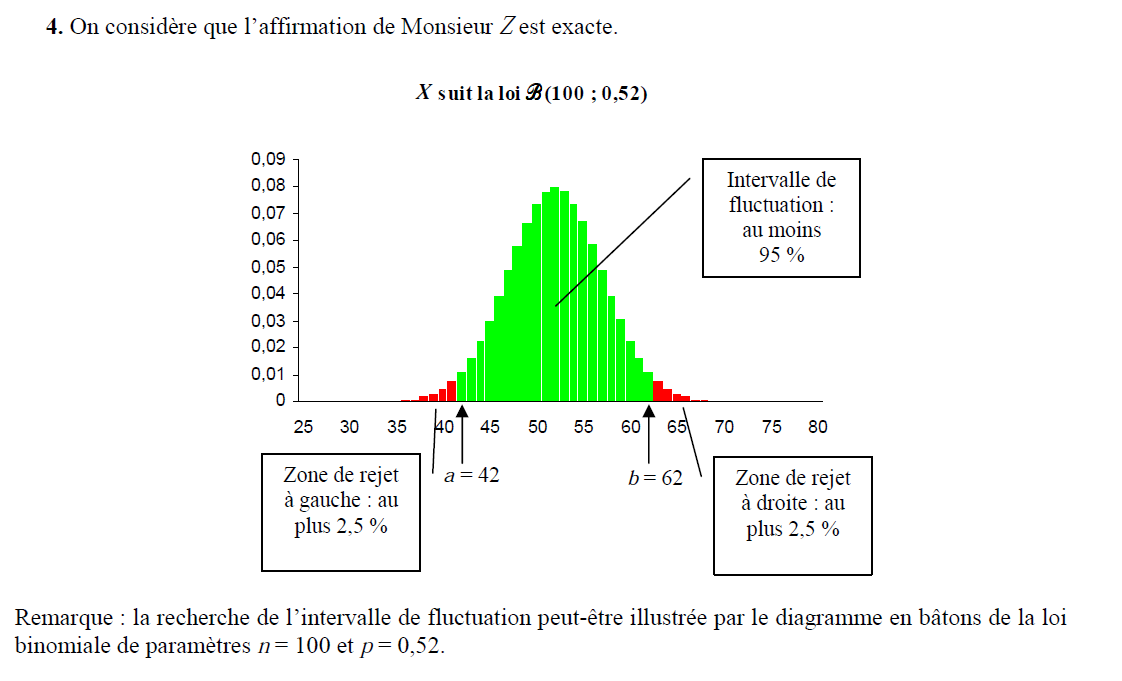
\includegraphics[scale=0.25]{corrige_exemple_decision2.png}
\end{center}

\end{frame}


\begin{frame}

Soit $X$ une variable aléatoire suivant la loi binomiale $\loibinom{100}{0,3}$.

Pour la variable aléatoire fréquence $\frac{X}{100}$, le programme ci-après donne l'intervalle de fluctuation exact au seuil de $95 \%$ :
\begin{equation*}
\Interff{\frac{21}{100}}{\frac{39}{100}}
\end{equation*}

\end{frame}

\begin{frame}

\frametitle{Intervalle de fluctuation exact, programme TI}


\texttt{\fbox{\textbf{Programme TEXAS}}\\ 
Prompt N \\
Prompt P \\
0$\rightarrow$ K\\
While binomFRep(N,P,K)$\leqslant$ 0.025\\
K+1$\rightarrow$K\\
End\\
Disp K\\
While binomFRep(N,P,K)$<$ 0.975\\
K+1$\rightarrow$K\\
End\\
Disp K\\
}


\end{frame}


\begin{frame}

\frametitle{Intervalle de fluctuation exact, programme CASIO}


\texttt{\fbox{\textbf{Programme CASIO}}\\ 
?$\rightarrow$ N \\
?$\rightarrow$ P \\
0$\rightarrow$ K\\
While binominalCD(K,N,P)$\leqslant$ 0.025\\
K+1$\rightarrow$K\\
WhileEnd\\
K \dispcasiotikz \\
While binominalCD(K,N,P)$<$ 0.975\\
K+1$\rightarrow$K\\
WhileEnd\\
K \dispcasiotikz \\
}


\end{frame}


\begin{frame}[fragile]
\frametitle{Intervalle de fluctuation exact, programme Python}


\begin{lstlisting}
from scipy.stats import binom

def binomFrep(n, p, k):
    """P(X <= k) si X suit  la loi  B(n,p)"""
    return binom.cdf(k, n, p)


def if_exact(n, p):
    k = 0
    while binomFrep(n, p, k) <= 0.025:
        k = k + 1
    binf = k
    while binomFrep(n, p, k) < 0.975:
        k = k + 1
    bsup = k
    return [binf, bsup]
\end{lstlisting}


\end{frame}


\begin{frame}
\label{exemple2}

\frametitle{Exemple 2 : Intervalle de fluctuation  exact}

Dans une maternité, on admet qu'il na\^it en moyenne 51 \% des garçons. On fait le point sur la proportion de garçons toutes les 100 naissances.

La  variable aléatoire $X$ donnant le nombre de garçons dans un échantillon de 100 naissances, suit une loi binomiale de paramètres $n=100$ et $p=0,51$, car nous sommes en présence d'une répétition de $100$ épreuves de Bernoulli identiques et indépendantes dont la probabilité de succès (naissance d'un garçon) est de $=0,51$.

Le programme réalisé à l'exemple $1$ retourne l'intervalle de fluctuation exact au seuil de $95 \%$ pour la fréquence $\frac{X}{100}$ de garçons  dans un échantillon de taille $n  = 100$ :
\begin{equation*}
\Interff{\frac{41}{100}}{\frac{61}{100}}
\end{equation*}


\end{frame}


\begin{frame}[fragile]

\frametitle{Exemple 2 : Intervalle de fluctuation  asymptotique (0/5)}

\begin{lstlisting}
from scipy.stats import  norm
from math import sqrt

def invNorm(s):
    """Retourne  u tel que que P(X <= u)= s si X suit la loi  N(0,1)"""
    return norm.ppf(s)


def if_asymptotique(n, p, s=0.95):
    u = invNorm((1 + s) / 2)
    binf = p - u * np.sqrt(p * (1 - p) / n)
    bsup = p + u * np.sqrt(p * (1 - p) / n)
    return [binf, bsup]
\end{lstlisting}

\end{frame}




\begin{frame}

\frametitle{Exemple 2 : Intervalle de fluctuation  asymptotique (1/5)}


Soit une  variable aléatoire $X_n$ suivant la loi binomiale $\loibinom{n}{p}$ avec $p$ dans l'intervalle $\Interoo{0}{1}$ et soit  \mbox{$\text{I}_n=\Interff{p-u_{\alpha}\frac{\sqrt{p(1-p)}}{\sqrt{n}}}{p+u_{\alpha}\frac{\sqrt{p(1-p)}}{\sqrt{n}}}$} \textbf{un intervalle de fluctuation \og{} asymptotique au seuil de  $1-\alpha$ \fg{}}  de la variable aléatoire fréquence $F_n=\frac{X_n}{n}$.

Sous les conditions,  $n \geqslant 30, \,   np \geqslant 5, \, n(1-p) \geqslant 5 
$ , on peut utiliser l'approximation $\proba{F_{n} \in \text{I}_n} \approx 1-\alpha$. Ainsi, l'intervalle de fluctuation asymptotique $\text{I}_n$ peut être considéré comme un intervalle de fluctuation de $F_{n}$ au seuil de $1-\alpha$.

\medskip

Un cas particulier important est celui de l'intervalle de fluctuation asymptotique au seuil de $0,95$ qui est\boldmath  $
\Interff{p-1,96\frac{\sqrt{p(1-p)}}{\sqrt{n}}}{p+1,96\frac{\sqrt{p(1-p)}}{\sqrt{n}}}$ \unboldmath.
\end{frame}


\begin{frame}

\frametitle{Exemple 2 : Intervalle de fluctuation  asymptotique (2/5)}

On considère ici une variable aléatoire suivant une loi binomiale $ \loibinom{100}{0,51}$.

Les conditions d'approximation usuelles sont vérifiées :

\begin{itemize}

	\item $n \geqslant 30$ car $n = 100$ ;
	
	\item $np \geqslant 5$ car $np = 100 \times 0,51 = 51$ ;
	
	\item $n(1-p) \geqslant 5$ car $n(1-p) = 100 \times 0,49 = 49$.
	
\end{itemize}

On peut donc utiliser l'intervalle de fluctuation asymptotique comme approximation d'un intervalle de fluctuation au seuil de $95 \%$ pour la variable aléatoire fréquence $\frac{X}{100}$ :
\begin{equation*}
\Interff{p-1,96\frac{\sqrt{p(1-p)}}{\sqrt{n}}}{p+1,96\frac{\sqrt{p(1-p)}}{\sqrt{n}}}
\end{equation*}

\end{frame}
 

\begin{frame}

\frametitle{Exemple 2 : Intervalle de fluctuation  asymptotique (3/5)}

En pratique on calcule l'intervalle de fluctuation asymptotique avec le programme ci-après (saisir $N=100$, $P= 0.51$ et $A=0.95$) et on obtient :

\begin{equation*}
\Interff{0,51-1,96\frac{\sqrt{0,51(1-0,51)}}{\sqrt{100}}}{0,51+1,96\frac{\sqrt{0,51(1-0,51)}}{\sqrt{100}}}
\end{equation*}
En arrondissant par défaut la borne inférieure et par excès la borne supérieure  à $0,001$ près : 
\begin{equation*}
\boxed{\Interff{0,412}{0,608}}
\end{equation*}

\end{frame}



\begin{frame}

\frametitle{Exemple 2 : Intervalle de fluctuation  asymptotique (4/5)}


\begin{center}
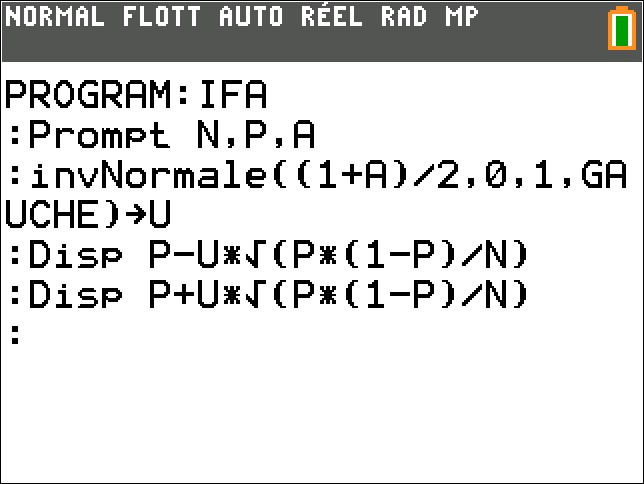
\includegraphics[scale=0.4]{IFA-TI.png}
\end{center}

\end{frame}



\begin{frame}

\frametitle{Exemple 2 : Intervalle de fluctuation  asymptotique (5/5)}

\begin{center}
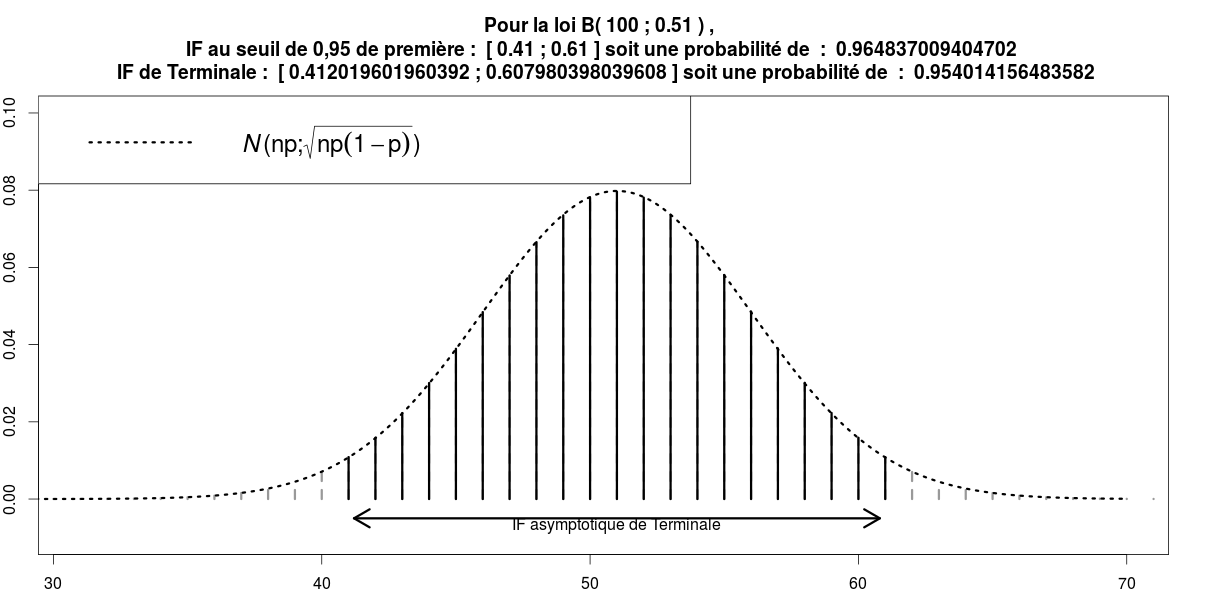
\includegraphics[scale=0.23]{IFA.png}
\end{center}

\end{frame}



\begin{frame}

\frametitle{Exemple 2 : Intervalles de fluctuation  asymptotique avec d'autres seuils que $0,95$}

La proportion d'un caractère dans une population  est $p=0,6$. Déterminons un intervalle de fluctuation asymptotique  de la fréquence de ce caractère dans les échantillons de taille 100, prélevés au hasard et avec remise :

\begin{enumerate}
\item au seuil de  $0,8$ : $\boxed{\Interff{0,537}{0,663}}$  ;
\item au seuil de  $0,9$ :  $\boxed{\Interff{0,519}{0,681}}$.
\end{enumerate}

\end{frame}


\begin{frame}
\frametitle{Exemple 3 Partie 1}

\label{exemple3} 

\begin{itemize}
\pause \item On s'intéresse au caractère \og{} Favorable à la coupure de l'éclairage nocturne \fg{} 
\pause \item On fait l'hypothèse que la proportion de ce caractère dans la population totale est de $p=0,5$.
\pause \item La taille de l'échantillon est $n=100$.
\pause \item Les conditions d'approximation usuelles $n \geqslant 30$, $np \geqslant 5$ et $n(1-p) \geqslant 5$ sont réunies et permettent d'utiliser $
\Interff{p-1,96\frac{\sqrt{p(1-p)}}{\sqrt{n}}}{p+1,96\frac{\sqrt{p(1-p)}}{\sqrt{n}}}$  comme intervalle de fluctuation asymptotique au seuil de $0,95$ de la fréquence  du caractère sur un échantillon de taille $n$.

\end{itemize}

\end{frame}




\begin{frame}
\frametitle{Exemple 3 Partie 2}



\begin{itemize}
\pause \item À $10^{-3}$ près un intervalle de fluctuation  asymptotique au seuil de $0,95$ de la fréquence  du caractère sur un échantillon de taille $n$ est $\Interff{0,402}{0,598}$.

\pause \item La fréquence mesurée sur l'échantillon est de $0,54$, elle est largement à l'intérieur de l'intervalle de fluctuation donc on peut accepter l'hypothèse que la proportion du caractère dans la population est $p=0,5$.

\end{itemize}

\end{frame}




\begin{frame}
\frametitle{Exemple 4 Partie 1}

\label{exemple4} 

\begin{itemize}
\pause \item On s'intéresse au caractère \og{} Conforme  \fg{}  d'un médicament produit.
\pause \item On fait l'hypothèse que la proportion de ce caractère dans la population totale est de $p=0,97$.
\pause \item La taille de l'échantillon est $n=1000$.
\pause \item Les conditions d'approximation usuelles $n \geqslant 30$, $np \geqslant 5$ et $n(1-p) \geqslant 5$ sont réunies et permettent d'utiliser $
\Interff{p-1,96\frac{\sqrt{p(1-p)}}{\sqrt{n}}}{p+1,96\frac{\sqrt{p(1-p)}}{\sqrt{n}}}$  comme intervalle de fluctuation asymptotique au seuil de $0,95$ de la fréquence  du caractère sur un échantillon de taille $n$.
\end{itemize}

\end{frame}



\begin{frame}
\frametitle{Exemple 4 Partie 2}



\begin{itemize}
\pause \item À $10^{-3}$ près un intervalle de fluctuation  asymptotique au seuil de $0,95$ de la fréquence  du caractère sur un échantillon de taille $n$ est $\Interff{0,959}{0,981}$.

\pause \item La fréquence mesurée sur l'échantillon est de $0,947$, elle est en dehors de l'intervalle de fluctuation donc on peut rejeter l'hypothèse que la proportion du caractère dans la population est $p=0,97$ avec un risque d'erreur (faux positif) de $0,05$.

\end{itemize}

\end{frame}




\begin{frame}
\frametitle{Exemple 5 Partie 1}

\label{exemple5}

Un institut effectue un sondage pour connaître, dans une population donnée, la proportion de personnes qui sont favorables à un projet d'aménagement du territoire. On interroge un échantillon aléatoire de $n$ personnes de cette population où $n$ est un entier naturel supérieur à 50.  Parmi ces personnes, une fréquence $f=0,29$ est  favorable au projet d'aménagement.



\begin{itemize}
\pause \item OLes conditions d'approximation usuelle $n \geqslant 30$, $nf \geqslant 5$ et $n(1-f) \geqslant 4$ sont vérifiées et permettent d'utiliser l'intervalle $\Interff{f-\frac{1}{\sqrt{n}}}{f+\frac{1}{\sqrt{n}}}$ pour estimer la probabilité du caractère dans la population totale au niveau de confiance $0,95$.
\pause \item L'amplitude de l'intervalle de confiance est $\frac{2}{\sqrt{n}}$. Le plus petit entier $n$ tel que  $\frac{2}{\sqrt{n}} \leqslant 0,04 \Leftrightarrow 50 \leqslant \sqrt{n} \Leftrightarrow 2500 \leqslant n$.
Le seuil recherché est donc $n=2500$.

\end{itemize}

\end{frame}



\end{document}